\documentclass[11pt,a4paper]{article}
\usepackage[margin=24mm,headheight=15pt]{geometry}
\usepackage[T1]{fontenc}
\usepackage{lmodern,microtype}
\usepackage{amsmath,amssymb,mathtools}
\usepackage{graphicx,tikz,pgfplots}
\usetikzlibrary{arrows.meta,positioning,calc}
\pgfplotsset{compat=1.18}
\usepackage{booktabs,tabularx,enumitem}
\usepackage{xcolor,fancyhdr,titlesec}
\definecolor{ink}{HTML}{17324D}
\definecolor{teal}{HTML}{087F8C}
\definecolor{orange}{HTML}{BD622A}
\definecolor{muted}{HTML}{526575}
\usepackage[colorlinks=true,linkcolor=teal,urlcolor=teal,citecolor=teal]{hyperref}
\hypersetup{pdftitle={What is quantum computing, and why does it matter?},pdfauthor={}}
\newcommand{\ket}[1]{\lvert #1\rangle}
\newcommand{\bra}[1]{\langle #1\rvert}
\newcommand{\ii}{\mathrm{i}}
\newcommand{\Prob}{\mathop{\mathrm{P}}}
\newcommand{\id}{\mathbb I}
\setlength{\parindent}{0pt}
\setlength{\parskip}{7pt}
\setlength{\emergencystretch}{2em}
\titleformat{\section}{\Large\bfseries\color{ink}}{\thesection}{0.6em}{}
\titleformat{\subsection}{\large\bfseries\color{ink}}{\thesubsection}{0.6em}{}
\pagestyle{fancy}\fancyhf{}
\fancyhead[L]{\small\color{muted} QUANTUM COMPUTING / FOUNDATIONS}
\fancyfoot[L]{\small\color{muted} Tutorial 01: Intro to Quantum Computing}
\fancyfoot[R]{\small\thepage}
\renewcommand{\headrulewidth}{0.3pt}
\setlist[itemize]{nosep,leftmargin=1.5em}
\newcommand{\takeaway}[1]{\begin{quote}\color{ink}\textbf{#1}\end{quote}}
\begin{document}
\begin{center}
{\small\color{teal}\textbf{PART OF A SERIES OF TUTORIALS ON QUANTUM ERROR CORRECTION}}\\[9pt]
{\LARGE\bfseries\color{ink} An Introduction to Quantum Computing}\\[10pt]
{\large What is quantum computing and why does it matter?}\\[9pt]
{\small 15 September 2026}
\end{center}
\vspace{3pt}
This tutorial assumes basic university-entry-level linear algebra, but no prior quantum mechanics or quantum computing. It prioritizes intuition over a fully rigorous mathematical or physical treatment.

We focus on pure states, ideal unitary operations, and projective measurements, leaving mixed states, noise, and generalized measurements for later. Geometric pictures and analogies serve as teaching aids rather than literal physical descriptions.

\section{Start with the familiar: computing}
To understand \emph{quantum computing}, let us separate the two words and start with the more familiar part. At an abstract level, a classical digital computer takes an input, applies a sequence of operations, and produces an output. We can represent its input and output as bit strings, for example:
\[
\underbrace{10011}_{\text{input}}
\quad\xrightarrow{\text{algorithm / operations}}\quad
\underbrace{11011}_{\text{output}}.
\]
The algorithm determines their actual relationship. Arithmetic such as addition and multiplication can be built from elementary logical operations, including AND and XOR. 
% Classical algorithms can also use randomness, so random output alone does not distinguish a quantum computer.

A quantum computer also prepares an input, applies operations, and obtains an output. In a
basic circuit description, its internal information is a quantum state, and its final readout is a
classical bit string:
\[
\ket{\psi_{\rm in}}
\quad\xrightarrow{\text{quantum operations}}\quad
\ket{\psi_{\rm out}}
\quad\xrightarrow{\text{measurement}}\quad
\text{classical bit string}.
\]

The key difference is how these physical systems represent and process information. A classical digital computer represents bits, \(0\) and \(1\), using distinguishable physical conditions---for example, voltage levels in transistor circuits. A quantum computer instead encodes information in \textbf{qubits} and preserves and controls their quantum states, allowing it to exploit effects beyond classical bit operations.



\section{What does ``quantum'' mean?}
The word \emph{quantum} comes from Latin and refers to an amount \cite{etymology}. The conventional starting point of quantum theory is Max Planck's work on thermal radiation in 1900, introducing energy elements proportional to frequency, $E=h\nu$, with $h$ now called Planck's constant \cite{planck}.

Discreteness is one consequence of quantum mechanics. An atom's bound states, for example, have specific allowed energies. This does not mean that every physical quantity always has a discrete spectrum. Quantum mechanics is a broader framework for states, their evolution, and measurement. For computing, its complex amplitudes and the ways they combine are especially important. In the rest of this article, we explore four ideas of quantum mechanics that are essential to quantum computing: superposition, measurement, interference, and entanglement.

\newpage
\section{Superposition: everything all at once}
A classical bit has value 0 or 1. For a qubit, we label two orthonormal basis states with the same symbols:
\begin{equation}
\ket{0}=\begin{pmatrix}1\\0\end{pmatrix},\qquad
\ket{1}=\begin{pmatrix}0\\1\end{pmatrix}.
\end{equation}
The symbol $\ket{\cdot}$, called a \emph{ket}, denotes a vector. These vectors form the computational basis, also called the $Z$ basis. A pure single-qubit state is a normalized linear combination:
\begin{equation}\label{eq:pure}
\ket{\psi}=\alpha\ket{0}+\beta\ket{1}
=\begin{pmatrix}\alpha\\\beta\end{pmatrix},\qquad
\alpha,\beta\in\mathbb C,\qquad |\alpha|^2+|\beta|^2=1.
\end{equation}
We call this a \emph{superposition\footnote{The word superposition may be familiar from Schr\"odinger's cat, often described as ``alive and dead at the same time.'' In the idealized thought experiment, the cat becomes entangled with a microscopic system, producing a joint superposition of two alternatives: an undecayed atom with a living cat, and a decayed atom with a dead cat. The puzzle is how this quantum description relates to the definite outcome we observe when we open the box.} in the chosen basis}. The coefficients $\alpha$ and $\beta$ are probability amplitudes. Generally, they are complex numbers and the sum of their squared magnitude equals 1. As we will see, these amplitudes can carry information that probabilities alone do not capture.

To expose that information, write $\alpha=r_0e^{\ii\gamma_0}$ and $\beta=r_1e^{\ii\gamma_1}$, with $r_0,r_1\geq0$. Then
\[
\ket{\psi}=e^{\ii\gamma_0}
\left(r_0\ket{0}+r_1e^{\ii(\gamma_1-\gamma_0)}\ket{1}\right).
\]
The prefactor is a \emph{global phase}. Multiplying a whole state by the same phase does not change its physical predictions (squared magnitude equals to 1). However, the relative phase $\phi=\gamma_1-\gamma_0$ can matter and will be discussed in Sec.\ref{sec: interference}. Normalization allows the parameterization
\begin{equation}\label{eq:blochstate}
\boxed{\ket{\psi}=\cos\frac\theta2\ket{0}
+e^{\ii\phi}\sin\frac\theta2\ket{1}},
\qquad 0\leq\theta\leq\pi,\quad 0\leq\phi<2\pi,
\end{equation}
up to global phase. At a pole, one component vanishes and $\phi$ does not distinguish states.

\subsection{A geometric picture: the Bloch sphere}
To help visualize the qubit, we can see that the two angles $\theta$ and $\phi$ identify a point on the surface of a unit sphere, what we call the \textbf{Bloch sphere}, with coordinates
\begin{equation}
\mathbf r=(\sin\theta\cos\phi,\ \sin\theta\sin\phi,\ \cos\theta)
\end{equation}
as the \textbf{Bloch vector} which represents the qubit state. On the Bloch sphere, the north pole represents $\ket{0}$, the south pole $\ket{1}$. The polar angle $\theta$ is measured down from $+Z$; the azimuth $\phi$ is measured around $Z$, from $+X$ toward $+Y$. Figure~\ref{fig:bloch} illustrates these coordinates.

There are two real degrees of freedom: the two complex coefficients in Eq.~\eqref{eq:pure} start with four real parameters, normalization removes one, and global phase removes another. However, a single measurement on one copy of an unknown quantum state cannot determine both angles \(\theta\) and \(\phi\). To understand what we can learn from a qubit, we must first discuss measurement.

\newpage
\begin{figure}[!ht]
\centering
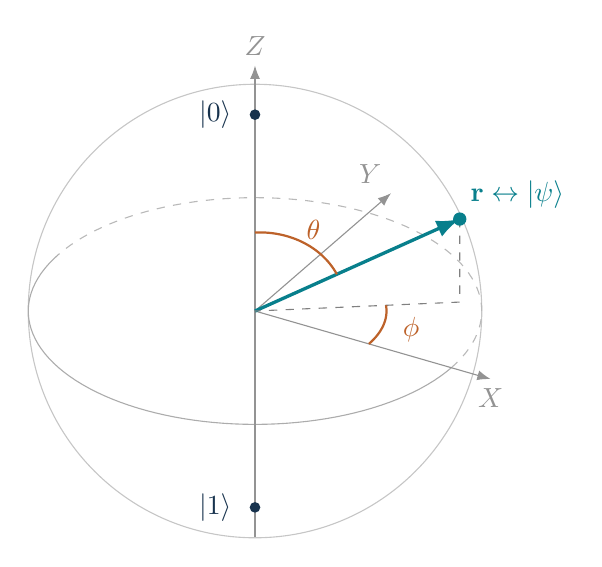
\begin{tikzpicture}[scale=1.20,>=Latex]
% Orthographic projection: screen coordinates of unit X,Y,Z.
\begin{scope}[x={(2.078cm,-.600cm)},y={(1.200cm,1.039cm)},z={(0cm,2.078cm)}]
\draw[gray!45] (0,0,0) circle[radius=2.4cm];
\draw[gray!55,dashed,domain=0:180,samples=70] plot ({cos(\x)},{sin(\x)},0);
\draw[gray!65,domain=180:360,samples=70] plot ({cos(\x)},{sin(\x)},0);
\draw[->,gray!85] (0,0,0)--(1.2,0,0) node[below] {$X$};
\draw[->,gray!85] (0,0,0)--(0,1.2,0) node[above left] {$Y$};
\draw[->,gray!85] (0,0,-1.15)--(0,0,1.25) node[above] {$Z$};
\coordinate (S) at ({sin(65)*cos(35)},{sin(65)*sin(35)},{cos(65)});
\coordinate (Q) at ({sin(65)*cos(35)},{sin(65)*sin(35)},0);
\draw[->,very thick,teal] (0,0,0)--(S) node[above right] {$\mathbf r\leftrightarrow\ket{\psi}$};
\draw[dashed,gray] (S)--(Q)--(0,0,0);
\draw[orange,thick,domain=0:65,samples=30] plot ({.40*sin(\x)*cos(35)},{.40*sin(\x)*sin(35)},{.40*cos(\x)});
\node[orange] at (.24,.1,.43) {$\theta$};
\draw[orange,thick,domain=0:35,samples=30] plot ({.58*cos(\x)},{.58*sin(\x)},0);
\node[orange] at (.68,.20,0) {$\phi$};
\fill[ink] (0,0,1) circle[radius=1.6pt] node[left=5pt] {$\ket{0}$};
\fill[ink] (0,0,-1) circle[radius=1.6pt] node[left=5pt] {$\ket{1}$};
\fill[teal] (S) circle[radius=2pt];
\end{scope}
\end{tikzpicture}
\caption{The Bloch sphere, shown in perspective. The sphere has unit radius; $\theta$ and $\phi$ locate a pure state. The dashed line drops to the equatorial plane. Bloch-space geometry and Hilbert-space state-vector projections are different constructions.}\label{fig:bloch}
\end{figure}

\section{Measurement: what can we observe?}
We begin with an \emph{ideal projective measurement in the computational basis}, the standard binary readout in a circuit model \footnote{Other measurements are possible, including measurements in different bases and generalized measurements (POVMs). By repeating the preparation and measuring in several bases, we can estimate \(\theta\) and \(\phi\); but no single measurement on one copy can reveal them completely.}. This measurement asks whether the outcome corresponds to \(\ket{0}\) or \(\ket{1}\); it does not report the state's coordinates on the Bloch sphere.

% The distinction is between a state and an outcome. The state determines the \emph{probabilities} of the possible outcomes, while one measurement produces just one outcome, labelled 0 or 1. Observing 0, for example, does not tell us whether its probability was \(1\), \(0.8\), or \(0.5\): many different initial states could have produced that result. Furthermore, computational-basis probabilities do not depend on the relative phase \(\phi\), so even repeated measurements in this basis cannot reveal it.

An ideal projective measurement also changes the state: conditional on obtaining outcome 0 or 1, the qubit is left in \(\ket{0}\) or \(\ket{1}\), respectively. Immediately repeating the same measurement therefore confirms that outcome rather than revealing more about the original state. To estimate both \(\theta\) and \(\phi\), we need many identically prepared copies and measurements in different bases.

The probability of each outcome is the squared magnitude of the overlap with its basis state. This is the \emph{Born rule}. A bra is the conjugate transpose of a ket, so
\[
\bra{0}=(1\;0),\qquad \bra{1}=(0\;1).
\]
For Eq.~\eqref{eq:blochstate},
\begin{align}
\Prob(0)&=|\bra{0}\psi\rangle|^2=\cos^2\frac\theta2,\\
\Prob(1)&=|\bra{1}\psi\rangle|^2=\sin^2\frac\theta2=1-\Prob(0).
\end{align}
The projections being squared are overlaps in the complex vector space of states. On the Bloch sphere, the vertical coordinate is instead $z=\cos\theta$, giving
\begin{equation}\label{eq:height}
\boxed{\Prob(0)=\frac{1+z}{2},\qquad\Prob(1)=\frac{1-z}{2}.}
\end{equation}
Thus the north pole yields 0 with certainty, the south pole yields 1 with certainty, and every equatorial state yields a 50--50 distribution. The Born rule supplies the physical probability law; the sphere visualizes it.

\newpage
\subsection{One result is not a description of the state}
If we obtain 0, we cannot tell whether its probability was $1$, $0.8$, or $0.5$. One result is a sample, not an estimate of the underlying distribution. Furthermore, $\phi$ does not appear in the computational-basis probabilities at all.

In an ideal projective measurement, the conditional state afterward is
\[
\ket{\psi}\longrightarrow
\begin{cases}
\ket{0},&\text{if the result is }0,\\
\ket{1},&\text{if the result is }1.
\end{cases}
\]
The Bloch vector ends at one of the two poles, not at its geometric projection somewhere along the axis. Immediately repeating the same measurement without intervening dynamics or noise returns the same result. To estimate the \emph{original} probabilities, we repeatedly prepare the same initial state and measure it.

Different measurement bases reveal different information. For a unit measurement axis $\mathbf n$, the two eigenvalue outcomes $\pm1$ have probabilities
\[
\Prob(\pm)=\frac{1\pm\mathbf r\cdot\mathbf n}{2}.
\]
For $Z$, the eigenvalues $+1,-1$ correspond to the bit labels $0,1$. Many identically prepared copies and several measurement settings let us estimate an unknown state. One copy cannot reveal an arbitrary state exactly: nonorthogonal states cannot be perfectly distinguished by any measurement.

More general measurements exist, but the projective model is sufficient for this introduction. We now have a more immediate question: \emph{if the $Z$ measurement does not see $\phi$, why include phase in the state at all?}

\section{Interference: making phase observable}\label{sec: interference}
\subsection{Split, accumulate phase, recombine}
A Ramsey-style experiment gives phase an operational meaning. We prepare $\ket{0}$, create two coherent components, let them acquire relative phase, and recombine them before measuring. For clean algebra, use the Hadamard gate
\begin{equation}
H=\frac1{\sqrt2}\begin{pmatrix}1&1\\1&-1\end{pmatrix},\qquad
H\ket{0}=\frac{\ket{0}+\ket{1}}{\sqrt2},\qquad
H\ket{1}=\frac{\ket{0}-\ket{1}}{\sqrt2}.
\end{equation}
An ideal closed-system gate is a unitary matrix, satisfying $U^\dagger U=\id$, which preserves normalization. The Hadamard is unitary and satisfies $H^2=\id$. It is \emph{not} a quarter-turn about $Y$: on the Bloch sphere, it is a half-turn about $(\hat{\mathbf x}+\hat{\mathbf z})/\sqrt2$.

Represent the relative-phase step by
\[
P_\phi=\begin{pmatrix}1&0\\0&e^{\ii\phi}\end{pmatrix}.
\]
A relative phase can build up during free evolution or be deliberately controlled. In physical Ramsey experiments, two $\pi/2$ pulses probe phase relative to a driving reference. Pulse phases and sign conventions can shift or invert the fringe. The $H$--$P_\phi$--$H$ sequence below is an idealized Ramsey-style version.

\newpage
\begin{figure}[!ht]
\centering
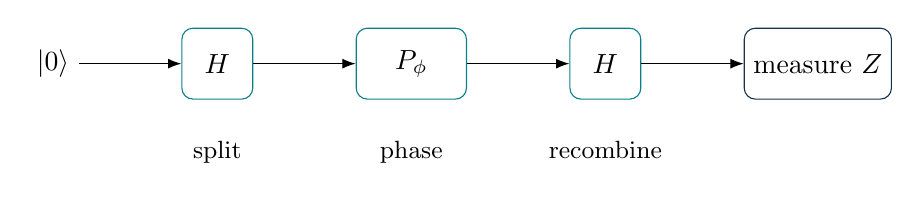
\begin{tikzpicture}[>=Latex,node distance=13mm]
\node (in) {$\ket{0}$};
\node[draw=teal,rounded corners,minimum size=9mm,right=of in] (h1) {$H$};
\node[draw=teal,rounded corners,minimum width=14mm,minimum height=9mm,right=of h1] (p) {$P_\phi$};
\node[draw=teal,rounded corners,minimum size=9mm,right=of p] (h2) {$H$};
\node[draw=ink,rounded corners,minimum height=9mm,right=of h2] (m) {measure $Z$};
\draw[->] (in)--(h1);\draw[->] (h1)--(p);\draw[->] (p)--(h2);\draw[->] (h2)--(m);
\node[below=4mm of h1,font=\small] {split};
\node[below=4mm of p,font=\small] {phase};
\node[below=4mm of h2,font=\small] {recombine};
\end{tikzpicture}
\caption{An idealized Ramsey-style sequence. The ``branches'' are internal-state amplitude components, not necessarily spatial paths.}
\end{figure}

The successive states are
\begin{align}
\ket{0}&\xrightarrow{H}\frac{\ket{0}+\ket{1}}{\sqrt2}
\xrightarrow{P_\phi}\frac{\ket{0}+e^{\ii\phi}\ket{1}}{\sqrt2},\\
\ket{\psi_{\rm out}}
&=\frac{H\ket{0}+e^{\ii\phi}H\ket{1}}{\sqrt2}\\
&=\frac{1+e^{\ii\phi}}2\ket{0}
+\frac{1-e^{\ii\phi}}2\ket{1}.\label{eq:out}
\end{align}
Before the second Hadamard, both populations are $1/2$, independently of $\phi$. After it, each output receives contributions from both intermediate components.

\begin{figure}[!ht]
\centering
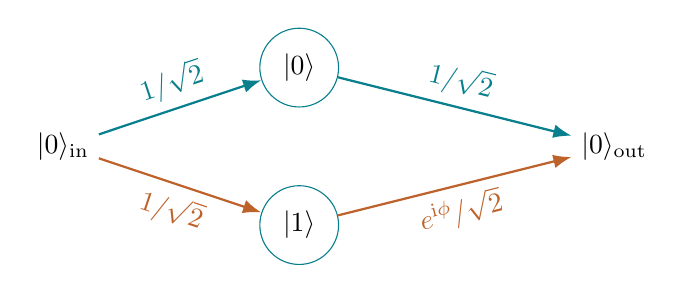
\begin{tikzpicture}[>=Latex]
\node (s) at (0,0) {$\ket{0}_{\rm in}$};
\node[draw=teal,circle,minimum size=10mm] (a) at (3,1) {$\ket{0}$};
\node[draw=teal,circle,minimum size=10mm] (b) at (3,-1) {$\ket{1}$};
\node (o) at (7,0) {$\ket{0}_{\rm out}$};
\draw[->,thick,teal] (s)--node[above,sloped] {$1/\sqrt2$}(a);
\draw[->,thick,orange] (s)--node[below,sloped] {$1/\sqrt2$}(b);
\draw[->,thick,teal] (a)--node[above,sloped] {$1/\sqrt2$}(o);
\draw[->,thick,orange] (b)--node[below,sloped] {$e^{\ii\phi}/\sqrt2$}(o);
\end{tikzpicture}
\caption{The two amplitude contributions to output 0. Multiply factors along each route, then add the routes: $A_0=1/2+e^{\ii\phi}/2$. The lower right edge includes phase accumulation and recombination. These are coherent alternatives, not measured trajectories.}\label{fig:paths}
\end{figure}

\subsection{Why this is interference}
Think of $1/2$ and $e^{\ii\phi}/2$ as arrows in the complex plane. When $\phi=0$, they point in the same direction and add to 1. When $\phi=\pi$, they point in opposite directions and add to 0. Intermediate phases give partial reinforcement or cancellation. At output 1, the relative minus sign reverses the pattern.

This is interference because the probability depends on the \emph{relative alignment} of amplitude contributions to the same outcome, not just their individual magnitudes. The input coefficients of $\ket{0}$ and $\ket{1}$ cannot simply cancel each other: they multiply different basis vectors. The second pulse brings their contributions into shared outputs.

\newpage
\subsection{The fringe: phase becomes a probability}
Using $e^{\ii\phi}+e^{-\ii\phi}=2\cos\phi$,
\begin{align}
\Prob(0)&=\frac{|1+e^{\ii\phi}|^2}{4}
=\frac{(1+e^{\ii\phi})(1+e^{-\ii\phi})}{4}
=\boxed{\frac{1+\cos\phi}{2}},\\
\Prob(1)&=\frac{|1-e^{\ii\phi}|^2}{4}
=\boxed{\frac{1-\cos\phi}{2}}.
\end{align}
The familiar general identity exposes the interference term:
\[
|a+b|^2=|a|^2+|b|^2+\underbrace{2\operatorname{Re}(a^*b)}_{\text{interference term}}.
\]
For reference, Feynman's treatment develops this amplitude-addition rule through alternative routes in an experiment \cite{feynman}.

\begin{figure}[!ht]
\centering
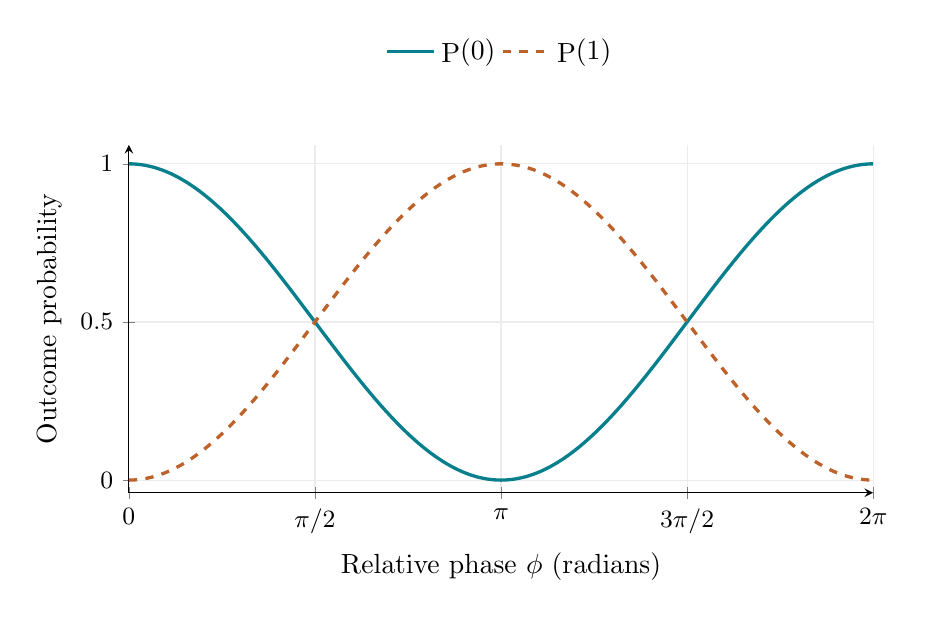
\begin{tikzpicture}
\begin{axis}[width=.91\linewidth,height=6cm,xmin=0,xmax=360,ymin=-.04,ymax=1.06,
xtick={0,90,180,270,360},xticklabels={$0$,$\pi/2$,$\pi$,$3\pi/2$,$2\pi$},
ytick={0,.5,1},xlabel={Relative phase $\phi$ (radians)},ylabel={Outcome probability},
axis lines=left,grid=major,grid style={gray!15},legend style={at={(.5,1.20)},anchor=south,draw=none,legend columns=2},
tick label style={font=\small},samples=181]
\addplot[teal,very thick,domain=0:360] {(1+cos(x))/2};\addlegendentry{$\Prob(0)$}
\addplot[orange,very thick,dashed,domain=0:360] {(1-cos(x))/2};\addlegendentry{$\Prob(1)$}
\end{axis}
\end{tikzpicture}
\caption{Ideal Ramsey-style fringes. Each plotted value is a probability estimated experimentally from many fresh preparations at that phase, not a continuous-valued result from one measurement.}
\end{figure}

At $\phi=0$, output 0 is certain; at $\phi=\pi$, output 1 is certain. At $\phi=\pi/2$, both are equally likely. As the relative phase changes, measured frequencies oscillate. These are interference fringes.

The role of coherence can be tested conceptually. If the components acquire a uniformly random, unrecorded relative phase before recombination, averaging gives $\langle\cos\phi\rangle=0$. The fringe disappears and both outcomes have probability $1/2$. An equal incoherent mixture behaves differently from a phase-controlled superposition.

\takeaway{Interference converts relative phase into observable probability differences. In sensing, the phase can encode a physical quantity; in an algorithm, it can encode information about a problem.}
One measurement setting does not identify phase uniquely: here $\phi$ and $2\pi-\phi$ have the same statistics. Other reference settings and repeated preparations provide additional information. Nor does a one-qubit interference experiment itself establish a computational speedup.

\newpage
\section{Entanglement: the state belongs to the pair}
With two qubits, a new question appears: can we always describe the pair by assigning each qubit its own pure state? If so, the joint state is a tensor product:
\begin{align}
\ket{\psi}_A\otimes\ket{\phi}_B
&=(a\ket{0}+b\ket{1})\otimes(c\ket{0}+d\ket{1})\\
&=ac\ket{00}+ad\ket{01}+bc\ket{10}+bd\ket{11}.
\end{align}
Here $\ket{xy}=\ket{x}_A\otimes\ket{y}_B$. Quantum mechanics also permits the Bell state
\begin{equation}\label{eq:bell}
\boxed{\ket{\Phi^+}=\frac{\ket{00}+\ket{11}}{\sqrt2}.}
\end{equation}
If this were a product, its coefficients would satisfy
\[
ac=bd=\frac1{\sqrt2},\qquad ad=bc=0.
\]
The first conditions require all four factors to be nonzero, contradicting the second conditions. No such factorization exists. This is the definition of \emph{entanglement for a bipartite pure state}.

The pair has a pure joint state, while neither member has its own pure state. Individual descriptions are still possible, but do not specify the full joint state. Entanglement is not a physical tether, an emotional bond, or a way to send a message through a parallel universe.

\subsection{More than matching results}
Measuring both qubits of Eq.~\eqref{eq:bell} in the $Z$ basis gives
\[
\Prob(00)=\Prob(11)=\tfrac12,\qquad
\Prob(01)=\Prob(10)=0.
\]
Each result is random, but the pair agrees. Agreement alone is not enough to demonstrate entanglement: randomly preparing either $\ket{00}$ or $\ket{11}$ gives the same statistics in this basis.

The difference is the coherent relative amplitude. Defining $\ket{\pm}=(\ket{0}\pm\ket{1})/\sqrt2$, we find
\[
\ket{++}+\ket{--}=\ket{00}+\ket{11},\qquad
\ket{\Phi^+}=\frac{\ket{++}+\ket{--}}{\sqrt2}.
\]
The Bell state's results also agree when both are measured in the $X$ basis. By contrast, the random preparation of $\ket{00}$ or $\ket{11}$ gives all four $X$-basis outcome pairs with probability $1/4$. This comparison distinguishes the Bell state from that classical mixture; a full Bell-inequality experiment requires further measurement choices.

If A measures $Z$ and obtains 0, the conditional state assigned to B is $\ket{0}$; if A obtains 1, it is $\ket{1}$. Without A's outcome, B still sees the same local 50--50 statistics. A cannot select the random outcome or signal instantly to B. Ordinary communication is needed to compare their records.

\takeaway{Entanglement concerns the full structure of a joint quantum state. Matching results in just one basis do not capture that structure.}

\newpage
\section{Putting the four ideas to work}
For $n$ qubits, a pure state has amplitudes over $2^n$ computational-basis strings:
\begin{equation}
\ket{\psi}=\sum_{x=0}^{2^n-1}\alpha_x\ket{x},\qquad
\sum_x|\alpha_x|^2=1.
\end{equation}
This does not provide $2^n$ freely readable answers. Preparing arbitrary amplitudes can itself be expensive, and a computational-basis measurement produces one string. Superposition supplies coherent amplitude components, not a list we can inspect simultaneously.

Under a unitary operation $U$, the output amplitude for $y$ is
\begin{equation}
\beta_y=\sum_x U_{yx}\alpha_x,\qquad \Prob(y)=|\beta_y|^2.
\end{equation}
Interference is explicit in this sum. Contributions from different $x$ reinforce or cancel. A quantum algorithm exploits the structure of a problem to make the measured results informative; it does not know the correct answer beforehand. Entanglement allows the joint state to extend beyond independent qubit descriptions. Measurement supplies the classical results, often through repeated runs and classical processing.

These ingredients must be used efficiently. State preparation, gates, error correction, repetitions, and readout all contribute to cost. Some circuits containing superposition, interference, and entanglement can still be simulated efficiently classically. Their mere presence does not guarantee an advantage.

\section{Why does quantum computing matter?}
The promise is not that quantum computers will improve every everyday task. It is that some important tasks may require substantially fewer computational resources. In the standard models, quantum computing changes questions of efficiency, not the boundary between computable and uncomputable problems.

\subsection{Scientific discovery}
Quantum systems are a natural application. Describing strongly interacting particles can be very costly classically; a controllable quantum processor offers another way to study quantum dynamics \cite{preskill}. Better calculations of molecules and materials could support research in catalysis and materials science, although translating a simulation into a useful product remains a substantial task \cite{doe}.

\subsection{Cybersecurity}
A sufficiently capable fault-tolerant quantum computer could break widely used public-key systems such as RSA and elliptic-curve cryptography. This motivates preparation now, including post-quantum cryptography: algorithms running on classical computers designed to resist quantum attacks \cite{pqc}.

Quantum cryptography, including quantum key distribution, is a related but distinct field. It uses quantum systems for cryptographic tasks and does not generally require a universal quantum computer \cite{qcrypto}. It should not be presented as an automatic security upgrade delivered by building one.

\newpage
\subsection{Engineering capacity and strategic investment}
Building quantum computers also drives work on demanding engineering problems. Concrete examples include cryogenic electronics for qubit control and readout \cite{cryo}; single-photon detectors shared with quantum networking and faint-light sensing \cite{detectors}; and low-noise measurement systems relevant to quantum processors and precision instruments \cite{readout}. These are mutually supporting developments across research fields, rather than inventions attributable solely to quantum computing.

Governments invest in potential computational capabilities, security preparedness, skilled workforces, and industrial capacity. The US National Quantum Strategy, for example, includes science, workforce, industry, infrastructure, economic security, and international cooperation \cite{strategy}. Quantum funding also supports sensing and networking; not every quantum investment is a computing investment \cite{nqi}.

\section{From quantum computing to error correction}
We can now give a more informative definition. A quantum computer processes information by controlling quantum states, their amplitudes, and their joint correlations, then extracts results through measurement. Relative phase matters because operations can turn it into probability differences. Entanglement matters because the information can belong to a joint state rather than a collection of independent pure states.

These capabilities create an engineering requirement: the useful quantum structure must survive long enough to complete the computation. Uncontrolled interactions, inaccurate gates, and imperfect readout can corrupt it. Our next topics examine what a qubit is physically, how circuits control it, and how error correction protects quantum information without simply reading out the information being protected.

\bigskip
\hrule
\medskip
\textbf{Questions to check your understanding}
\begin{enumerate}[leftmargin=1.5em]
\item Why can two equatorial states have identical $Z$-measurement probabilities while being different states?
\item In the Ramsey-style sequence, what happens at $\phi=0$ and at $\phi=\pi$? Which amplitude contributions cancel?
\item Why does measuring a qubit repeatedly after one projective measurement not estimate its original state?
\item What distinguishes the Bell state from a random preparation of $\ket{00}$ or $\ket{11}$?
\item Why does a state with $2^n$ amplitudes not guarantee an exponential computational advantage?
\end{enumerate}

% \newpage
% \appendix
% \section{Editorial notes: changes to the spoken draft}
% \textit{This appendix is for the author. It can be removed without changing the tutorial. The points below flag corrected claims and resolve places where the narration was uncertain.}

% \subsection*{History and terminology}
% \textbf{Corrected:} ``Quantum is Greek and means discrete.'' It is Latin and refers to an amount. Planck's 1900 thermal-radiation work is the conventional starting point for quantum theory, not the first use of the word in any context. The atom example is qualified as \emph{bound-state} energies: not every spectrum is discrete.

% \subsection*{State parameters and phase}
% \textbf{Clarified:} Amplitudes \emph{can} be complex; real amplitudes are allowed. A pure qubit has two real degrees of freedom after normalization and global phase are removed. The relative phase is meaningful when both components are present; at the poles its coordinate is redundant. Mixed states are acknowledged but deferred.

% \subsection*{Measurement and projection}
% \textbf{Corrected:} Squaring a Bloch-vector projection does not give the Born-rule probability. The squared quantity is the state-vector overlap $|\bra{m}\psi\rangle|^2$. On the Bloch sphere, $\Prob(0)=(1+z)/2$. An ideal projective measurement leaves a pole state, not a point partway along the axis. One copy cannot determine an arbitrary state; many fresh copies and measurement settings can estimate it.

% \subsection*{Hadamard versus a quarter-turn}
% \textbf{Corrected:} $H$ is not $R_y(\pi/2)$. Up to global phase, it is a Bloch rotation by $\pi$ about $(X+Z)/\sqrt2$, and $H^2=\id$. If the lecture instead uses two same-direction $Y$ quarter-turns, the fringe is inverted: without an intervening phase, $R_y(\pi/2)^2\ket{0}=\ket{1}$. Do not mix that geometry with the $H$--$P_\phi$--$H$ formulas.

% \subsection*{What makes interference visible}
% \textbf{Expanded:} The recombination diagram identifies two contributions to one output. Phase changes their sum. ``Coherent probabilities'' becomes ``coherent amplitude components.'' Inferring phase requires repeated measurements and, for an unambiguous estimate, suitable additional settings. The Ramsey description is explicitly idealized; physical pulse conventions differ.

% \newpage
% \subsection*{Entanglement and analogies}
% \textbf{Replaced:} Couples, twins, and physical attachment suggest misleading classical or signalling pictures. The essay uses nonfactorization and a Bell-state example. The product criterion applies to pure states. For mixed states, separability means a probabilistic mixture of product density matrices; entangled mixed states lack such a decomposition. Individual subsystems can be described, but those descriptions do not contain the full joint information.

% \subsection*{Computation and motivation}
% \textbf{Qualified:} ``All answers at once'' becomes amplitudes over basis strings, with no promise of reading all of them or obtaining a speedup. ``Previously unsolvable'' becomes potentially more resource-efficient for particular tasks. The cybersecurity discussion separates code-breaking, post-quantum cryptography, and quantum key distribution. Engineering examples are identified as shared developments, not guaranteed spin-offs caused solely by quantum computing.

% \section{Reference notes}
% Sources support historical, application, and policy claims. The state-vector calculations are worked explicitly in the essay. Web references were consulted in September 2026; policy and technology context should be reviewed before publication. Link titles below are clickable.

\begin{thebibliography}{99}\small
\bibitem{etymology} Online Etymology Dictionary. \href{https://www.etymonline.com/word/quantum}{``Quantum.''}
\bibitem{planck} NobelPrize.org. \href{https://www.nobelprize.org/prizes/themes/the-nobel-prize-in-physics-1901-2000/}{The Nobel Prizes in Physics 1901--2000.}
\bibitem{feynman} R. P. Feynman, R. B. Leighton, and M. Sands. \emph{The Feynman Lectures on Physics}, Vol. III, Chapter 3: \href{https://www.feynmanlectures.caltech.edu/III_03.html}{Probability Amplitudes.}
\bibitem{preskill} J. Preskill (2021). \href{https://arxiv.org/abs/2106.10522}{Quantum computing 40 years later.} arXiv:2106.10522.
\bibitem{doe} US Department of Energy. \href{https://www.energy.gov/science/bes/articles/connected-moments-and-quantum-computing-improve-many-body-chemical-simulations}{Connected Moments and Quantum Computing Improve ``Many Body'' Chemical Simulations.}
\bibitem{pqc} NIST. \href{https://www.nist.gov/cybersecurity-and-privacy/what-post-quantum-cryptography}{What Is Post-Quantum Cryptography?}
\bibitem{qcrypto} NIST. \href{https://www.nist.gov/cybersecurity-and-privacy/what-quantum-cryptography}{What Is Quantum Cryptography?}
\bibitem{cryo} NIST. \href{https://www.nist.gov/programs-projects/flux-quantum-electronics}{Flux Quantum Electronics.}
\bibitem{detectors} NIST. \href{https://www.nist.gov/quantum-information-science/quantum-sensing-explained/seeing-bits-light}{Seeing Bits of Light.}
\bibitem{readout} NIST. \href{https://www.nist.gov/pml/quantum-sensors/quantum-electronics}{Quantum Electronics Group.}
\bibitem{strategy} National Quantum Initiative. \href{https://www.quantum.gov/strategy/}{National Quantum Strategy.}
\bibitem{nqi} National Quantum Initiative. \href{https://www.quantum.gov/national-quantum-initiative/}{The National Quantum Initiative.}
\end{thebibliography}
\end{document}
